\documentclass[10pt,conference]{IEEEtran}
\IEEEoverridecommandlockouts
\usepackage{cite}
\usepackage{amsmath,amssymb,amsfonts}
\usepackage{algorithmic}
\usepackage{graphicx}
\usepackage{textcomp}
\usepackage{xcolor}
\usepackage{booktabs}
\usepackage{url}
\usepackage{tikz}
\usetikzlibrary{positioning,arrows.meta,calc}
\setlength{\textfloatsep}{4pt plus 1pt minus 2pt}
\setlength{\floatsep}{3pt plus 1pt minus 1pt}
\setlength{\dbltextfloatsep}{4pt plus 1pt minus 2pt}
\setlength{\dblfloatsep}{3pt plus 1pt minus 1pt}
\setlength{\abovecaptionskip}{3pt}
\setlength{\belowcaptionskip}{1pt}
\setlength{\abovedisplayskip}{4pt plus 1pt minus 2pt}
\setlength{\belowdisplayskip}{4pt plus 1pt minus 2pt}

\def\BibTeX{{\rm B\kern-.05em{\sc i\kern-.025em b}\kern-.08em
    T\kern-.1667em\kern-.125emX}}

\begin{document}

\title{NetOpsAgent: A Hierarchical Multi-Agent LLM Framework for Autonomous Cloud Infrastructure Incident Management}

\author{\IEEEauthorblockN{Kinjal Vaishnav}
\IEEEauthorblockA{Oracle Cloud Infrastructure, Seattle, WA, USA \\
kinjal.vaishnav@oracle.com}
}

\maketitle

\begin{abstract}
Cloud infrastructure incidents cause significant service disruption, yet mean
time to root cause remains long due to alert volume and telemetry complexity.
We present NetOpsAgent, a hierarchical multi-agent LLM framework for
autonomous cloud incident management, decomposing investigation into four
agents---Supervisor, Telemetry, Reasoning, Action---coordinated via a shared
\texttt{InvestigationState} object, with a confidence-gated tiered autonomy
mechanism bounding autonomous-action risk. We evaluate on two independent
real fault-injection benchmarks: AIOps Challenge 2020 (N=75) and RCAEval RE1
(N=75). Across six pre-registered configurations---including a raw-context
fix, RAG with and without relevance gating, and a test designed specifically
to isolate decomposition's benefit---we find no statistically significant
multi-agent advantage over a single-agent baseline on either dataset
(McNemar $p>0.05$ throughout), and a rule-based baseline stays competitive
with both. We then test a targeted extension: a Falsifier agent adversarially
validating the Reasoning agent's hypothesis against evidence it did not
use, mirroring the validation mechanism recent RCA multi-agent systems
report gains from. This significantly improves accuracy on single-entity
incidents (33.3\% vs.\ 21.3\%, $p=0.023$) but significantly regresses
multi-service incidents (24.0\% vs.\ 42.7\%, $p<0.001$): the extension
lacks service-dependency-graph awareness and mistakes a downstream symptom
for the root cause once more than one service is involved. Adding real service-topology data eliminates
the regression ($p=0.50$, was $p<0.001$) but does not yet produce a gain
there. A control test shows the AIOps gain comes from the Falsifier
capability itself, not the decomposition it was attached to: the same
Falsifier on a single-agent hypothesis scores statistically
indistinguishably from the multi-agent version ($p=1.0$ head-to-head). We
report this in full, characterize why self-reported LLM confidence fails
to support safe autonomous action here, and identify the likely mechanism
(blind metric selection under decomposition) behind the base
architecture's underperformance. A reference implementation is publicly
available under the MIT license.
\end{abstract}

\begin{IEEEkeywords}
multi-agent LLM systems, AIOps incident management, autonomous root cause
analysis, site reliability engineering, retrieval-augmented generation
\end{IEEEkeywords}

\section{Introduction}
\label{sec:intro}

Site reliability engineering in large-scale cloud environments faces a
structural tension: incident frequency scales with system complexity, but
human investigation capacity does not, and mean time to root cause for
complex distributed failures commonly exceeds 30--60 minutes
\cite{beyer2016sre,lim2018oncall}. LLMs offer a qualitatively different
approach: instruction following, tool use, and multi-step reasoning over
unstructured text make them natural candidates for investigation tasks
historically requiring senior engineers. Yet naive single-agent application
fails in practice---the context window fills with raw telemetry before the
model can reason causally, with no principled mechanism for deciding when
confidence is sufficient to act autonomously.

We present NetOpsAgent, a hierarchical multi-agent LLM framework
addressing both limitations, decomposing investigation into four
specialized agents---Supervisor, Telemetry Investigation, Reasoning,
Action---each handling a distinct phase of the response workflow. A shared
\texttt{InvestigationState} object propagates structured findings between
agents, enforcing context hygiene without information loss, and a
confidence-gated tiered autonomy mechanism lets the system act
autonomously on high-confidence hypotheses while escalating uncertain
cases to humans.

The framework targets two observed single-agent failure modes.
\emph{Context pollution}: given access to all observability tools, a single
agent accumulates raw metrics, logs, and configuration data in one context
window, too large and heterogeneous for reliable causal reasoning,
particularly where the causal signal is weak relative to background noise.
\emph{Uncalibrated autonomy}: without principled confidence scoring, an LLM
agent takes either too many autonomous actions (increasing blast radius) or
too few (eliminating the productivity benefit). NetOpsAgent is designed to
address both; Section~\ref{sec:eval} reports how well that design holds up
under controlled measurement.

This paper makes four contributions: (1) the NetOpsAgent architecture and its
design rationale; (2) a controlled empirical evaluation across two independent
real datasets and six architectural configurations, showing that multi-agent
decomposition and retrieval augmentation do not produce a significant
improvement over a single-agent baseline for this task---including under a
test designed specifically to favor the multi-agent hypothesis; (3) a
failure-mode and confidence-calibration analysis, including a real finding
that self-reported and self-consistency LLM confidence both fail to
discriminate correct from incorrect hypotheses in this setting; and (4) a
targeted extension experiment adding a Falsifier/validation agent, showing a
statistically significant improvement on single-entity incidents and a
statistically significant regression on multi-service incidents, with the
divergence traced to a specific, addressable mechanism (missing
service-dependency-graph awareness) rather than left as an unexplained split.

\section{Related Work}
\label{sec:related}

\subsection{LLM Agents and Tool Use}
ReAct \cite{yao2023react} established the observe-reason-act loop as the
foundational pattern for LLM agents with external tool access. Subsequent
work---Toolformer \cite{schick2023toolformer}, function-calling APIs such as
Gorilla \cite{patil2023gorilla}---showed LLMs reliably invoke structured
tools given well-defined schemas. LangGraph \cite{langgraph2024} introduced
stateful, cyclical agent graphs with persistent state across tool
invocations; NetOpsAgent builds directly on this, using LangGraph's
\texttt{StateGraph} as the orchestration primitive.

\subsection{AIOps, Benchmarks, and Multi-Agent Coordination}
Classical network anomaly detection relies on threshold alerting,
statistical process control, and ML classifiers on labeled KPI time series
\cite{zhao2020aiops}, consistent with standardized observability data
formats \cite{opentelemetry2024}; the wider AIOps landscape spans log
parsing \cite{liu2023logprompt} to runbook execution \cite{winters2020seag},
typically rule-based or ML pipelines with limited cross-incident-type
generalization. NetOpsAgent consumes the alert these systems produce as
input and addresses the investigation phase that follows. SWE-bench
\cite{jimenez2024swebench,jimenez2024swebenchverified} evaluates agents on
asynchronous software tasks; our evaluation (Section~\ref{sec:eval})
instead draws ground-truth labels directly from AIOps Challenge 2020
\cite{zhao2020aiops} and RCAEval, rather than constructing author-labeled
traces. On LLM-based RCA: Guo et al.\ \cite{guo2023chatgptevent} apply
GPT-4 to log parsing with strong zero-shot but limited causal reasoning;
Chen et al.\ \cite{chen2024eurosys} propose trace-based LLM RCA for
microservices; Luo et al.\ \cite{luo2022issre} use a knowledge-graph
approach; Roy et al.\ \cite{roy2024llmrca} describe single-agent RAG-based
triage. NetOpsAgent differs in hierarchical decomposition, confidence-gated
tiered autonomy, and an ablation measuring decomposition's own contribution
(Section~\ref{sec:eval}). LLM-based multi-agent coordination itself differs
from classical MAS research in using natural language and JSON rather than
formal ontologies: AutoGen \cite{wu2023autogen} and MetaGPT
\cite{hong2023metagpt} show conversational patterns solve software
engineering tasks in low-risk settings, while NetOpsAgent targets
reliability-critical contexts---typed state propagation, confidence-gated
action safety, full audit logging; Section~\ref{sec:eval} evaluates how
much the first of these actually contributes on real data.

\subsection{Positioning Relative to Recent RCA Multi-Agent Systems}
\label{sec:novelty}
Two recent systems decompose RCA into specialized LLM agents and ground
hypotheses in retrieved external knowledge, much as NetOpsAgent does.
Flow-of-Action \cite{pei2025flowofaction} pairs a main investigation agent
with auxiliary agents that retrieve, generate, and execute SOP steps,
reporting 64.01\% root-cause accuracy vs.\ a 35.50\% ReAct baseline on its
own industrial benchmark. MA-RCA \cite{fu2026marca} separates a Retrieval
Agent (RAG grounding) from a Validation Agent (dynamic-testing
verification), reporting 95.2\% F1 on Nezha and 82.8\% F1 on a
power-metering dataset.

NetOpsAgent's four-agent decomposition---Supervisor, Telemetry
Investigation, Reasoning, Action, with RAG inside the Reasoning agent---is
an instance of the same general pattern: specialize by cognitive function,
ground reasoning in retrieved precedent, keep verification structurally
separate from generation where possible. We do not claim architectural
novelty over Flow-of-Action or MA-RCA, and have narrowed this paper's
contribution accordingly.

This paper instead contributes a controlled empirical comparison, under
matched task, telemetry, and LLM backbone conditions, of whether that
general pattern outperforms a single well-prompted agent on two
independent real datasets. Section~\ref{sec:eval} finds decomposition
alone does not, unlike the substantial gains Flow-of-Action and MA-RCA
report on their own benchmarks. We go further and test MA-RCA's specific
mechanism---a dedicated validation stage---directly against our data
(Section~\ref{sec:falsifier}): it helps on single-entity incidents and,
without service-topology awareness, hurts on multi-service ones---a
falsifiable account of \emph{when} this pattern pays off, not a blanket
negative or unqualified replication.

This null result is consistent with concurrent findings outside RCA: Xu et
al.\ \cite{xu2026rethinking} show \emph{homogeneous} multi-agent
workflows (agents sharing one base model) are matched by a single
well-tuned agent and argue a real advantage needs \emph{heterogeneous}
models---NetOpsAgent already satisfies that (GPT-4o for Reasoning,
GPT-4o-mini for Telemetry, Section~\ref{sec:impl}) and still shows no gain;
Su and Wu \cite{su2026outperform} explain why theoretically---decomposition
helps for \emph{independent} subtasks and loses its advantage as they
become interdependent, closer to whole-incident diagnosis, consistent with
the blind-metric-selection mechanism in Section~\ref{sec:discussion}.A.

\subsection{Confidence Estimation in LLM Systems}
Verbalized confidence elicitation---asking the model for a numeric score
in the spirit of chain-of-thought prompting \cite{wei2022cot}---correlates
with accuracy on some factual tasks, though calibration degrades
out-of-distribution \cite{guo2017calibration}. In SRE, an overconfident
incorrect hypothesis can trigger autonomous actions that extend an
incident. Section~\ref{sec:eval} measures this directly: verbalized
confidence does not separate correct from incorrect hypotheses here, and
self-consistency fails for the same reason---an open problem, not a solved
one.

\section{Framework Architecture}
\label{sec:arch}

\subsection{System Overview}
NetOpsAgent comprises four agents coordinated via a LangGraph
\texttt{StateGraph}. All agents share a single \texttt{InvestigationState}
\texttt{TypedDict} that accumulates findings, tool results, and confidence
scores across the investigation lifecycle. The Supervisor Agent acts as the
graph entry point and routing controller; the three worker
agents---Telemetry Investigation, Reasoning, and Action---are dispatched
sequentially or conditionally based on Supervisor routing decisions.

This is a hierarchical, not linear-pipeline, architecture: the Supervisor
does not simply hand off to the next stage in a fixed sequence---it
classifies each incident, generates the routing plan the Telemetry Agent
executes, and retains authority to interrupt or redirect the pipeline
mid-investigation (Section~\ref{sec:arch}.C). Control flows top-down from
Supervisor to worker agents, while data flows bottom-up through
\texttt{InvestigationState} back to where routing decisions are
made---the defining property of a hierarchical, versus strictly
sequential, design.

A central design principle is context hygiene via decomposition: each agent
receives only the information relevant to its task, not the full raw
telemetry stream. The Telemetry Agent receives the alert trigger and
produces structured findings; the Reasoning Agent receives those findings
(not raw tool responses) and produces a hypothesis; the Action Agent
receives the hypothesis and confidence score. This staged flow is intended
to prevent context pollution from degrading reasoning quality, tested
directly in Section~\ref{sec:eval}. Fig.~\ref{fig:arch} shows the full
architecture.

\begin{figure*}[t]
\centering
\resizebox{0.98\textwidth}{!}{%
\hyphenpenalty=10000
\exhyphenpenalty=10000
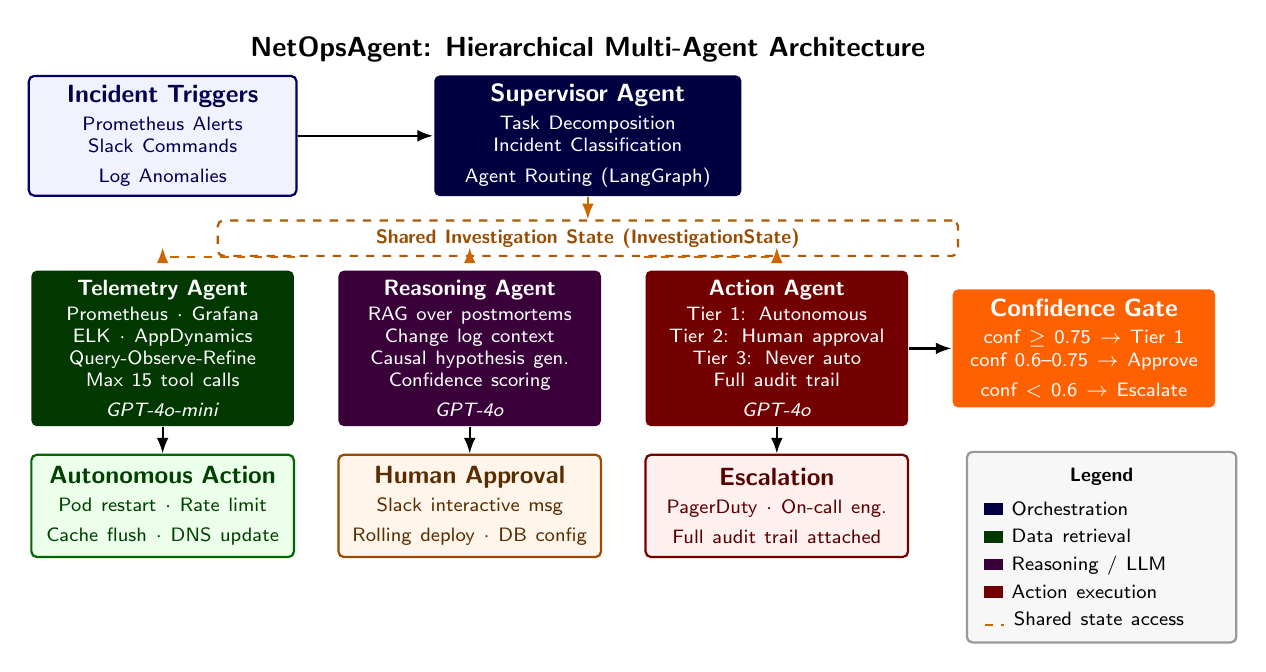
\begin{tikzpicture}[
  font=\sffamily\small,
  every node/.style={align=center},
  box/.style={rectangle, rounded corners=2pt, minimum width=3.4cm, minimum height=1.5cm, text width=3.1cm, draw, thick},
  arr/.style={-{Latex[length=2mm]}, thick},
  darr/.style={-{Latex[length=2mm]}, thick, dashed, color=orange!80!black}
]

\node[font=\sffamily\bfseries\normalsize] at (5.4,6.5) {NetOpsAgent: Hierarchical Multi-Agent Architecture};

\node[box, draw=blue!40!black, fill=blue!5, text=blue!30!black] (trig) at (0,5.4)
  {\textbf{\color{blue!30!black}Incident Triggers}\\[2pt]\scriptsize Prometheus Alerts\\ \scriptsize Slack Commands\\ \scriptsize Log Anomalies};

\node[box, draw=none, fill=blue!25!black, text=white, text width=3.6cm, minimum width=3.9cm] (sup) at (5.4,5.4)
  {\textbf{Supervisor Agent}\\[2pt]\scriptsize Task Decomposition\\ \scriptsize Incident Classification\\ \scriptsize Agent Routing (LangGraph)};

\draw[arr] (trig.east) -- (sup.west);

\node[box, draw=orange!70!black, dashed, fill=white, minimum width=9.4cm, text width=9.2cm, minimum height=0.45cm, inner sep=1pt] (state) at (5.4,4.1)
  {\scriptsize\textbf{\color{orange!60!black}Shared Investigation State (InvestigationState)}};

\draw[darr] (sup.south) -- (state.north);

\node[box, draw=none, fill=green!22!black, text=white, minimum width=3.2cm] (tel) at (0,2.7)
  {\footnotesize\textbf{Telemetry Agent}\\[1pt]\scriptsize Prometheus $\cdot$ Grafana\\ \scriptsize ELK $\cdot$ AppDynamics\\ \scriptsize Query-Observe-Refine\\ \scriptsize Max 15 tool calls\\ \scriptsize\textit{GPT-4o-mini}};

\node[box, draw=none, fill=violet!45!black, text=white, minimum width=3.2cm] (rea) at (3.9,2.7)
  {\footnotesize\textbf{Reasoning Agent}\\[1pt]\scriptsize RAG over postmortems\\ \scriptsize Change log context\\ \scriptsize Causal hypothesis gen.\\ \scriptsize Confidence scoring\\ \scriptsize\textit{GPT-4o}};

\node[box, draw=none, fill=red!45!black, text=white, minimum width=3.2cm] (act) at (7.8,2.7)
  {\footnotesize\textbf{Action Agent}\\[1pt]\scriptsize Tier 1: Autonomous\\ \scriptsize Tier 2: Human approval\\ \scriptsize Tier 3: Never auto\\ \scriptsize Full audit trail\\ \scriptsize\textit{GPT-4o}};

\node[box, draw=none, fill=orange!75!red, text=white, minimum width=3.2cm] (gate) at (11.7,2.7)
  {\textbf{Confidence Gate}\\[2pt]\scriptsize conf $\geq$ 0.75 $\to$ Tier 1\\ \scriptsize conf 0.6--0.75 $\to$ Approve\\ \scriptsize conf $<$ 0.6 $\to$ Escalate};

\draw[darr] (tel.north east|-state.south) -| ($(tel.north)+(0,8pt)$);
\draw[darr] (rea.north|-state.south) -- ($(rea.north)+(0,8pt)$);
\draw[darr] (act.north west|-state.south) -| ($(act.north)+(0,8pt)$);
\draw[arr] (act.east) -- (gate.west);

\node[box, draw=green!40!black, fill=green!8, text=green!25!black, minimum width=3.2cm, minimum height=1.3cm] (auto) at (0,0.7)
  {\textbf{\color{green!25!black}Autonomous Action}\\[2pt]\scriptsize Pod restart $\cdot$ Rate limit\\ \scriptsize Cache flush $\cdot$ DNS update};

\node[box, draw=orange!60!black, fill=orange!8, text=orange!35!black, minimum width=3.2cm, minimum height=1.3cm] (appr) at (3.9,0.7)
  {\textbf{\color{orange!35!black}Human Approval}\\[2pt]\scriptsize Slack interactive msg\\ \scriptsize Rolling deploy $\cdot$ DB config};

\node[box, draw=red!45!black, fill=red!6, text=red!35!black, minimum width=3.2cm, minimum height=1.3cm] (esc) at (7.8,0.7)
  {\textbf{\color{red!35!black}Escalation}\\[2pt]\scriptsize PagerDuty $\cdot$ On-call eng.\\ \scriptsize Full audit trail attached};

\draw[arr] (tel.south) -- (auto.north);
\draw[arr] (rea.south) -- (appr.north);
\draw[arr] (act.south) -- (esc.north);

\node[rectangle, rounded corners=2pt, draw=black!40, thick, fill=black!3, text width=3.0cm, inner sep=6pt, anchor=north west] (leg) at (10.2,1.4) {
\begin{minipage}{3.0cm}
\centering{\bfseries\scriptsize Legend}\\[4pt]
\raggedright\scriptsize
\tikz\fill[blue!25!black,sharp corners] (0,0) rectangle (0.25,0.15); Orchestration\\[2pt]
\tikz\fill[green!22!black,sharp corners] (0,0) rectangle (0.25,0.15); Data retrieval\\[2pt]
\tikz\fill[violet!45!black,sharp corners] (0,0) rectangle (0.25,0.15); Reasoning / LLM\\[2pt]
\tikz\fill[red!45!black,sharp corners] (0,0) rectangle (0.25,0.15); Action execution\\[2pt]
{\color{orange!80!black}\tikz\draw[dashed,thick] (0,0.07) -- (0.25,0.07);} Shared state access
\end{minipage}
};

\end{tikzpicture}%
}
\caption{NetOpsAgent hierarchical multi-agent architecture for autonomous
cloud network incident management. The Supervisor Agent routes incoming
alerts to the Telemetry Investigation Agent, which executes iterative tool
calls against mocked observability APIs. Structured findings propagate to the
Reasoning Agent, which applies chain-of-thought reasoning and RAG retrieval to
generate a root cause hypothesis with a confidence score. The Action Agent
dispatches remediation actions according to the confidence-gated three-tier
autonomy model. All agents share a single \texttt{InvestigationState} object.
}
\label{fig:arch}
\end{figure*}

\subsection{InvestigationState Schema}
All agents communicate exclusively via a shared \texttt{InvestigationState}
\texttt{TypedDict} with key fields
\texttt{alert\_trigger} (External: type, service, severity),
\texttt{routing\_plan} (Supervisor: ordered tool query plan),
\texttt{findings} (Telemetry: typed signal/value/timestamp list),
\texttt{rag\_context} (Reasoning: top-5 postmortem chunks),
\texttt{hypothesis} (Reasoning: root cause + mechanism),
\texttt{confidence} (Reasoning: float [0,1]),
\texttt{actions\_taken} (Action: dispatched action log), and
\texttt{tool\_errors} (Telemetry: schema/timeout failures). This enforces
strict information boundaries---no agent reads another's internal
context---intended to prevent the context accumulation failure mode seen
in single-agent baselines, and provides a natural audit log: the final
state records every finding, hypothesis, and action decision.

\subsection{Supervisor Agent}
The Supervisor Agent receives the alert trigger, classifies the incident
by layer (network, infrastructure, application) and severity, generates a
routing plan for the Telemetry Agent, and can interrupt or redirect the
pipeline if intermediate findings indicate a change in scope.

\subsection{Telemetry Investigation Agent}
The Telemetry Investigation Agent executes iterative tool calls against
mocked observability APIs---Prometheus \cite{rabenstein2015prometheus}
(metrics), ELK \cite{elastic2024elasticsearch} (logs), and a CMDB---in a
ReAct loop (querying, observing partial results, forming follow-up queries)
until it assembles sufficient evidence or exhausts its query budget. Its
output is a structured findings object appended to
\texttt{InvestigationState}: a typed list of (signal, value, timestamp,
significance) tuples, not raw API responses---the primary mechanism
controlling context size between agents.

\subsection{Reasoning Agent}
The Reasoning Agent receives structured findings from the Telemetry Agent
and generates a root-cause hypothesis using chain-of-thought prompting
\cite{wei2022cot} and RAG \cite{lewis2020rag}, querying a FAISS
\cite{johnson2021faiss} vector index of historical postmortems for
precedent cases similar to the current findings. Output is a hypothesis
tuple: (root\_cause, mechanism, confidence\_score, supporting\_evidence,
contradicting\_evidence). The confidence score (0--1) comes from a
structured self-evaluation prompt rating evidence quality, hypothesis
specificity, and absence of contradicting signals, and drives the
downstream action-safety gate; Section~\ref{sec:eval} evaluates how well it
actually does so.

\subsection{Action Agent and Confidence Gate}
The Action Agent implements a three-tier autonomy model keyed on hypothesis
confidence:
\begin{itemize}
  \item \textbf{Tier 1} ($c \geq 0.75$): Low-risk corrective actions (BGP
  timer adjustments \cite{bjorklund2011netconf}, instance restarts, cache
  flushes) executed autonomously.
  \item \textbf{Tier 2} ($0.6 \leq c < 0.75$): Medium-risk actions
  (configuration changes, traffic rerouting) queued for human approval with a
  pre-populated runbook suggestion.
  \item \textbf{Tier 3} ($c < 0.6$): High-risk actions (data migrations,
  teardowns) never executed autonomously; human operator notified with full
  investigation context.
\end{itemize}
All actions, autonomous and queued, are logged to
\texttt{InvestigationState} with the full hypothesis evidence chain for
post-incident audit.

\subsection{Falsifier Extension (Evaluated Separately from the Base Design)}
\label{sec:falsifier-arch}
Section~\ref{sec:eval} additionally evaluates an optional fifth agent, a
Falsifier, inserted between Reasoning and Action. Unlike the four agents
above, it is not part of the base architecture evaluated in
Sections~\ref{sec:eval}.A--F; we describe and evaluate it
separately in Section~\ref{sec:falsifier} since its contribution depends on
incident structure in a way the base components do not. The Falsifier
receives the Reasoning agent's hypothesis with the complete raw evidence
pool, including signals its summary did not surface, and is prompted to
actively look for contradicting evidence rather than confirm the
hypothesis, returning a
\texttt{confirmed}/\texttt{contested}/\texttt{refuted} verdict; a
\texttt{refuted} verdict with a concrete, better-supported alternative
overrides the hypothesis before Action acts. This mirrors the \emph{role}
of MA-RCA's Validation Agent \cite{fu2026marca}, not its mechanism: MA-RCA
executes dynamic checks against the system, ours only re-examines existing
telemetry via an LLM call---a cheaper, weaker proxy for the same role.

\section{Implementation}
\label{sec:impl}

\subsection{Technology Stack}
The prototype is implemented in Python 3.11: LangGraph 0.1 for
orchestration, Google ADK for tools. GPT-4o \cite{openai2023gpt4} drives
Supervisor and Reasoning; GPT-4o-mini drives Telemetry Investigation.
Section~\ref{sec:eval} reports measured, not anecdotal, latency and cost.
Model assignment follows cost/latency-vs-stakes: Telemetry issues up to 15
tool calls per investigation so cost/latency compound with volume, while
Supervisor and Reasoning each make one higher-stakes call---hence
GPT-4o-mini for telemetry, GPT-4o for supervision/reasoning. The
model-choice ablation supports this: GPT-4o-mini matches GPT-4o on AIOps,
trails on RCAEval, at roughly one-seventeenth the per-token cost.

\subsection{Observability Tool Layer}
Observability APIs are mocked via a deterministic trace-replay layer
emitting realistic metric/log responses from stored scenarios. Tool
failures surface as structured exceptions (e.g., ``Prometheus query timed
out after 10s; returned data covers 60\% of requested window'') so the
agent reasons about incompleteness rather than crashing.

\subsection{RAG Index Construction}
The Reasoning Agent retrieves historical incident context via vector
similarity search: postmortems chunked (512 tokens, 64-token overlap),
embedded with \texttt{text-embedding-3-small} (1,536 dims
\cite{devlin2019bert}), stored in a FAISS flat index
\cite{johnson2021faiss}. The agent retrieves the top-5 most similar chunks
by cosine similarity, with recency decay ($\lambda=0.95$/month) applied
before ranking. Section~\ref{sec:eval} evaluates a generic,
incident-independent version with and without relevance gating.

\subsection{Tool Validation and Error Handling}
A three-layer strategy handles errors: tool calls validated against JSON
Schema before execution (schema); timeouts capped per class (Prometheus
10s, ELK 15s, CMDB 5s, execution); failures logged to
\texttt{InvestigationState} and surfaced to the Supervisor for compensating
routing (state).

\subsection{Code Availability}
The extraction pipeline and evaluation harness producing every Section~V
result---incident extraction, all six configurations, the Falsifier
extension, topology-aware fix, single-agent control, raw per-incident
outputs---is available at
\url{https://github.com/Kinjal-Oza/multi-agent-observability-demo} under
the MIT license: the summary-based harness used for evaluation, not a full
iterative tool-calling deployment against live APIs.

\section{Evaluation}
\label{sec:eval}

\subsection{Dataset Construction}
We evaluate on two independent real datasets, rather than one real dataset
plus author-constructed synthetic scenarios as in our original submission.
\textbf{AIOps Challenge 2020}: 81 ground-truth incidents from the public KPI
dataset \cite{zhao2020aiops}, 75 usable after requiring a valid
pre-incident baseline window (6 excluded); labels come directly from
published anomaly annotations, no author-assigned labels. \textbf{RCAEval
RE1} (Zenodo, CC-BY-4.0): 75 independent fault-injection scenarios across
three real microservice systems (Online Boutique, Sock Shop, Train Ticket),
one run per unique service$\times$fault-type combination of six repeated
runs each ships with, avoiding pseudoreplication; ground truth is the
dataset's own injected fault label. Both datasets carry externally
published ground truth, so this revision no longer needs the
author-assigned synthetic labels and inter-rater reliability check
($\kappa$) \cite{cohen1960kappa} from the original submission's 80-trace
synthetic set---a source of potential labeling bias this design removes
rather than mitigates.

\subsection{Baselines}
Two baselines are evaluated on each dataset: the \emph{single-agent
baseline} receives the same alert trigger and tool schema as NetOpsAgent
but runs as one GPT-4o agent without decomposition, same task description
and completion condition (hypothesis with confidence score)---directly
testing decomposition's contribution; the \emph{rule-based baseline}
implements a fixed-heuristic classifier on metric-threshold crossing, a
pre-LLM production approach.

\subsection{Architectural Configurations Evaluated}
Six configurations were run once each on each dataset, pre-registered
before execution so the reported outcome could not be selected after the
fact:
\begin{enumerate}
  \item \textbf{Baseline} multi-agent (mini-summary $\to$ reasoning).
  \item \textbf{Sort-fix}: rank findings by relative deviation from
  baseline, not raw magnitude (AIOps only).
  \item \textbf{Raw-context fix}: the Reasoning Agent sees raw signal data,
  not only the Telemetry Agent's summary.
  \item \textbf{+RAG}: real embeddings (\texttt{text-embedding-3-small}), a
  21-chunk generic operational-knowledge corpus, top-5 retrieval.
  \item \textbf{+RAG, gated}: as above, restricted to cosine similarity
  $\geq 0.45$ (threshold fixed from a diagnostic sample before this
  ablation, not tuned to its outcome).
  \item \textbf{Fair context-pollution test}: single-agent gets a true
  unranked, unfiltered raw telemetry dump (this paper's definition of
  context pollution); multi-agent's Telemetry Agent performs real
  iterative, blind metric-name-based selection first (this paper's
  definition of context hygiene via decomposition)---the only configuration
  testing either side against the architecture's own motivating hypothesis.
\end{enumerate}
The generic RAG corpus (Section~\ref{sec:impl}) contains 21 chunks of
general SRE knowledge (CPU, memory, disk, network-delay, network-loss,
database-layer triage), authored before any evaluation ran, with no
incident-specific text---independence from the evaluation traces is true by
construction and verifiable by inspection, not merely asserted.

\subsection{Results}
Table~\ref{tab:results} reports exact-match accuracy for every
configuration on both datasets. McNemar's test \cite{mcnemar1947test} on
discordant pairs returns $p>0.05$ for every configuration on both datasets
except the fair context-pollution test ($p<0.001$), significant
\emph{favoring the single agent}---opposite the paper's original
hypothesis.

\begin{table}[h]
\caption{Exact-match accuracy, both datasets (N=75 each)}
\label{tab:results}
\centering
\footnotesize
\begin{tabular}{lcccc}
\toprule
& \multicolumn{2}{c}{AIOps 2020} & \multicolumn{2}{c}{RCAEval RE1} \\
Configuration & Single & Multi & Single & Multi \\
\midrule
Baseline & 24.0\% & 17.3\% & 41.3\% & 34.7\% \\
Sort-fix & 20.0\% & 18.7\% & --- & --- \\
Raw-context fix & 22.7\% & 22.7\% & 33.3\% & 37.3\% \\
+RAG & 24.0\% & 24.0\% & 29.3\% & 34.7\% \\
+RAG, gated & 22.7\% & 25.3\% & 29.3\% & 30.7\% \\
Fair test\footnotemark[1] & 25.3\% & 4.0\% & --- & --- \\
Rule-based\footnotemark[2] & \multicolumn{2}{c}{76.0\%} & 36.0\% & --- \\
\bottomrule
\end{tabular}
\footnotetext[1]{Raw dump (single) vs.\ iterative blind selection (multi); AIOps only.}
\footnotetext[2]{Fault-type match only, not comparable to root-cause-and-mechanism matching.}
\end{table}

\textbf{No configuration shows a statistically significant multi-agent
advantage on either dataset.} A rule-based baseline is competitive with, or
beats, both LLM architectures on AIOps, where the rule-based classifier's
76.0\% is roughly 3x every LLM configuration's accuracy---a practical
answer for a deploying team: nothing here argues for replacing a working
heuristic with an LLM pipeline on this task today. Two reviewer-requested ablations produced small, real,
secondary effects: RAG relevance gating reduced a CPU/disk over-retrieval
bias (67/75$\to$59/75 guesses mentioning CPU or disk regardless of true
cause), modestly improving AIOps accuracy; GPT-4o-mini, in the
single-agent role, matched GPT-4o on AIOps (22.7\% both) but trailed on
RCAEval (26.7\% vs.\ 33.3\%) (cost detail in Section~\ref{sec:impl}).

\subsection{Confidence Calibration}
\label{sec:confidence}
Verbalized self-reported confidence does \emph{not} discriminate correct
from incorrect hypotheses: mean confidence for incorrect hypotheses is
nearly identical to correct ones on both datasets (AIOps, $N{=}75$: 0.86
correct vs.\ 0.85 incorrect; RCAEval: 0.90 vs.\ 0.87), and at the proposed
0.75 gate, 96--100\% of incorrect hypotheses would pass in both---the same
rate as correct ones. Self-consistency confidence (5 resamples, temperature
0.7, majority-vote, fixed $N{=}30$ AIOps subsample) also fails (0.98
correct vs.\ 0.93 incorrect): the model is frequently \emph{consistently}
wrong---the same error repeats across resamples, a systematic-bias failure
resampling cannot fix, unlike sampling-noise miscalibration---a real,
publishable safety finding about the limits of LLM confidence gating here,
not a gap to paper over.

\subsection{Latency, Cost, and Threshold Sensitivity}
\label{sec:latency}
On a 15-incident sample, measured (not estimated) wall-clock latency and
OpenAI published per-token cost were 0.75s / \$0.0013 single-agent vs.\
3.53s / \$0.0010 multi-agent---the summary-based harness used throughout,
not a full iterative tool-calling deployment against live APIs; the two are
not directly comparable, and we do not present these as a validated
production estimate. Separately, the rule-based baseline's CPU threshold
was swept 50--95\%: exact-or-partial accuracy ranged 73.3--81.3\%, highest
at the lowest threshold tried---not strongly sensitive to this choice
within a normal range, stated explicitly rather than presenting one
threshold as tuned.

\subsection{Falsifier Extension: A Conditional, Mechanistically-Explained Result}
\label{sec:falsifier}
None of the six configurations above give multi-agent a capability
single-agent could not also have; they only reorganize what Reasoning
sees. Flow-of-Action \cite{pei2025flowofaction} and MA-RCA
\cite{fu2026marca} report large gains from a genuinely new capability
instead (executable SOP grounding, or a dedicated Validation Agent testing
each hypothesis dynamically). We pre-registered a targeted test of an
LLM-based proxy for the latter (Section~\ref{sec:falsifier-arch}): add the
Falsifier to the raw-context-fix configuration, run once on both datasets,
report regardless of direction. Two implementation issues, found in a
pre-run smoke test before any accuracy number was computed, were fixed on
implementation grounds, not outcome grounds: free-text alternatives could
return a negation (``Low CPU Usage'') the keyword scorer misread as a
match, fixed by constraining alternatives to the closed vocabulary used
throughout; and the initial adversarial prompt refuted nearly every
hypothesis, including correct ones, fixed by requiring
\texttt{confirmed} as the default absent concrete contradicting evidence.

\begin{table}[h]
\caption{Falsifier extension: exact match, single run each dataset}
\label{tab:falsifier}
\centering
\resizebox{\columnwidth}{!}{%
\small
\begin{tabular}{lccc}
\toprule
Dataset (N=75) & Single-agent & +Falsifier & McNemar $p$ \\
\midrule
AIOps, multi-agent+Falsifier & 21.3\% & 33.3\% & 0.023 \\
AIOps, single-agent+Falsifier & 21.3\% & 32.0\% & 0.077 \\
RCAEval (multi-service) & 42.7\% & 24.0\% & $<0.001$ \\
RCAEval, topology-aware & 42.7\% & 40.0\% & 0.50 \\
\bottomrule
\end{tabular}%
}
\end{table}

The result is significant in both directions at once. On AIOps (single
entity), the extension corrected 11 wrong hypotheses and broke only 2
previously-correct ones---a significant improvement. On RCAEval (a real
microservice call graph per incident), it corrected \emph{zero} wrong
hypotheses and broke 12---a significant regression. Why: the Falsifier
repeatedly overrides a correct root-cause service with a \emph{different}
service also anomalous in the same window---textbook symptom propagation,
a downstream service degrading because of an upstream cause, not because
it is the cause. Lacking service-dependency-graph awareness, the Falsifier
cannot tell ``anomalous because it is the cause'' from ``anomalous because
it is a victim,'' impossible on AIOps, where there is only one entity to
reason about.

The AIOps result pairs the Falsifier with the multi-agent hypothesis,
leaving open whether the gain needs decomposition. A pre-registered control
isolates this: the same Falsifier on the (reused) single-agent hypothesis
scores 21.3\%$\to$32.0\%, $p=0.077$, almost identical to multi-agent
(33.3\%); a direct incident-level comparison returns $p=1.0$ (21 right
under both, 47 wrong under both, 4 vs.\ 3 on the rest)---statistically
indistinguishable. The Falsifier drives the AIOps gain, not the
decomposition it was attached to; crossing $p<0.05$ in one condition
reflects how close the estimates are, not a real architectural
difference. The same single-run caveat applies here: the 8-point sampling
swing in Section~\ref{sec:discussion}.B means this significance reflects
within-run pairing, not run-to-run reproducibility.

This is mechanistically explained: validation helps when the alternative
space is one entity's own metrics, and hurts when it spans a call graph
without topology awareness. We tested the fix directly: give the Falsifier
each system's real service dependency graph (verified for Online Boutique
and Sock Shop; a naming-convention proxy for Train Ticket's 64
services---so confirmed for two of three systems, Train Ticket's
contribution resting on an unverified proxy), instructing it that graph-connected
co-anomalies are expected propagation, not independent evidence. This eliminates the regression
(24.0\%$\to$40.0\%, indistinguishable from single-agent's 42.7\%,
$p=0.50$ vs.\ $p<0.001$ before) but adds no gain: the topology-aware
Falsifier made zero overrides across all 75 incidents, trading
overconfidence for near-total caution rather than discrimination---harm
fixed, value not yet added.

\section{Discussion}
\label{sec:discussion}

\subsection{Design Principles}
Three principles motivated the design; we revisit each against
Section~\ref{sec:eval}. \emph{Context hygiene via decomposition}: the fair
context-pollution test shows the clearest result, in the opposite
direction: blind, values-withheld metric-name selection defaults to
generic, dataset-typical names regardless of which signal is actually
anomalous, so Telemetry frequently investigates the wrong evidence before
Reasoning ever sees it---the actual finding, not the original unqualified
claim. \emph{Asymmetric safety calibration}: an incorrect autonomous
action extends an incident while an unnecessary escalation costs minutes,
arguing for conservative thresholds under SRE risk-budgeting
\cite{murphy2016embracingrisk}, independent of decomposition's benefit.
\emph{Observability}: full logging of every tool call, inference, and
state transition is what made Section~\ref{sec:confidence}'s
confidence-discrimination failure discoverable at all.
Section~\ref{sec:falsifier} sharpens this further: the capability helping
single-entity incidents did not need the decomposition it was attached to
($p=1.0$)---value comes from the capability, not agent count
(Section~\ref{sec:novelty}).

\subsection{Limitations and Threats to Validity}
The evaluation has several limitations. AIOps 2020 and RCAEval RE1 each
cover a specific set of systems and fault types that may not represent all
cloud environments; RCAEval's ground truth is an injected fault label, not
a full causal narrative, capping how finely ``exact match'' is defined,
and AIOps's annotations have an analogous limitation. Confidence
thresholds need recalibration against live data---Section~\ref{sec:confidence}
shows no threshold in the practical range currently discriminates safely.
All configurations ran once: re-running an \emph{unchanged} prompt moved
its own score by 8 points from sampling noise alone (RCAEval single-agent,
41.3\%$\to$33.3\%), larger than most reported effects; a repeated-run
protocol was not performed, so point estimates are indicative. On validity: the single-agent baseline uses the same tool
schema and prompt length, but both prompts were written by the same
author, a potential bias either way (\emph{internal}); results come from
two public benchmarks, so generalization elsewhere is plausible but
unconfirmed (\emph{external}); and ``partial match'' conflates cases of
varying operator usefulness, so the headline comparison uses exact match,
the stricter metric (\emph{construct}).

\subsection{Security and Deployment Considerations}
Autonomous LLM agents executing production remediations \cite{burns2016borg}
introduce a distinct security surface: prompt injection via telemetry
(mitigate by sanitizing tool-boundary inputs, treating outputs as data,
not instructions), confidence manipulation via a poisoned RAG index
(easier given Section~\ref{sec:confidence}'s weak confidence-correctness
link; mitigate via restricted write access and ingestion audits), and
audit-log integrity (\texttt{InvestigationState} should be append-only,
integrity-verified)---none disqualifies autonomous operation, but security
review is a prerequisite. Deployment raises further concerns: alert-burst
queuing (e.g., Alertmanager grouping); the 0.75 Tier~1 threshold should
not be adopted without re-running Section~\ref{sec:confidence}'s
discrimination analysis against a deployment's own history; GPT-4o
updates may shift calibration without notice, arguing for pinned versions
or an open model (Llama 3 \cite{meta2024llama3}); and the RAG index needs
active maintenance, since recency decay ($\lambda=0.95$/month) only
partially offsets staleness.

\subsection{Future Work}
Motivated by Section~\ref{sec:falsifier}: verify Train Ticket's full call
graph beyond the naming-convention proxy used here, and sharpen the
override decision. Beyond that: a production
evaluation with real incident data and fault-injection studies
\cite{basiri2016chaos}; a repeated-run protocol isolating real effects
from sampling noise; fine-tuning a smaller open model (Llama 3
\cite{meta2024llama3}) and re-measuring single- vs.\ multi-agent; and a
public benchmark on AIOps 2020/RCAEval against Flow-of-Action
\cite{pei2025flowofaction} and MA-RCA \cite{fu2026marca}.

\section{Conclusion}
\label{sec:conclusion}

We presented NetOpsAgent, a hierarchical multi-agent LLM framework for
autonomous cloud incident management, decomposing investigation into four
agents coordinated via a shared state object. On two independent real
fault-injection benchmarks (AIOps Challenge 2020, RCAEval RE1, $N=75$ each)
across six configurations, decomposition did not significantly improve on
a single-agent baseline, including under a configuration designed
specifically to test the architecture's own context-hygiene hypothesis---an
honest, triangulated finding that multi-agent LLM decomposition's benefit
for infrastructure triage is more setup-dependent than prior work
(Flow-of-Action \cite{pei2025flowofaction}, MA-RCA \cite{fu2026marca}) has
reported. We also found, and report in full, that neither verbalized nor
self-consistency-based confidence discriminates correct from incorrect
hypotheses here, materially limiting the safety guarantee our
confidence-gated autonomy mechanism can currently provide.

Finally, a targeted Falsifier extension adversarially validating the
Reasoning agent's hypothesis---mirroring the validation mechanism recent
multi-agent RCA systems report gains from---produced a real, significant
effect in both directions: improving accuracy on single-entity incidents
(AIOps), degrading it on multi-service incidents (RCAEval), because
without service-dependency-graph awareness it mistakes propagated symptoms
for root causes once an incident spans more than one service. A
service-topology fix (Section~\ref{sec:falsifier}) removes the RCAEval
regression but does not yet turn it into a gain---honest, not rounded up.
A control test shows the AIOps gain does not require decomposition: a
single agent given the same Falsifier scores indistinguishably from
multi-agent ($p=1.0$). This
paper's central claim is therefore not that multi-agent architecture adds
value for LLM-based RCA, but that a specific \emph{capability}---adversarial
verification---does, independent of agent count. Practically: skip
decomposition, invest in adversarial verification with topology awareness,
and confirm an LLM pipeline earns its complexity over a heuristic. All findings are reported
because a verification or autonomy mechanism is only useful if its
failure modes are visible; the public implementation and harness make
all of them, and any future re-measurement, reproducible.

\section*{Acknowledgment}
The author thanks the LangGraph and Google ADK communities.

\begin{thebibliography}{00}
\footnotesize
\renewcommand{\baselinestretch}{0.83}\selectfont
\setlength{\itemsep}{0pt}\setlength{\parskip}{0pt}\setlength{\parsep}{0pt}

\bibitem{beyer2016sre} B. Beyer, C. Jones, J. Petoff, and N. R. Murphy, \emph{Site Reliability Engineering: How Google Runs Production Systems}. O'Reilly, 2016.
\bibitem{yao2023react} S. Yao et al., ``ReAct: Synergizing reasoning and acting in language models,'' in \emph{Proc. ICLR}, 2023.
\bibitem{schick2023toolformer} T. Schick et al., ``Toolformer: Language models can teach themselves to use tools,'' in \emph{Proc. NeurIPS}, 2023.
\bibitem{langgraph2024} LangChain Team, ``LangGraph: Building stateful, multi-actor applications with LLMs,'' 2024.
\bibitem{zhao2020aiops} J. Zhao et al., ``AIOps Challenge 2020: KPI anomaly detection,'' 2020.
\bibitem{wei2022cot} J. Wei et al., ``Chain-of-thought prompting elicits reasoning in large language models,'' in \emph{Proc. NeurIPS}, 2022.
\bibitem{wu2023autogen} Q. Wu et al., ``AutoGen: Enabling next-gen LLM applications via multi-agent conversation,'' arXiv:2308.08155, 2023.
\bibitem{hong2023metagpt} S. Hong et al., ``MetaGPT: Meta programming for multi-agent collaborative framework,'' arXiv:2308.00352, 2023.
\bibitem{patil2023gorilla} S. Patil et al., ``Gorilla: Large language model connected with massive APIs,'' arXiv:2305.15334, 2023.
\bibitem{jimenez2024swebench} C. Jimenez et al., ``SWE-bench: Can language models resolve real-world GitHub issues?'' in \emph{Proc. ICLR}, 2024.
\bibitem{devlin2019bert} J. Devlin et al., ``BERT: Pre-training of deep bidirectional transformers for language understanding,'' in \emph{Proc. NAACL}, 2019.
\bibitem{johnson2021faiss} J. Johnson, M. Douze, and H. J\'egou, ``Billion-scale similarity search with GPUs,'' \emph{IEEE Trans. Big Data}, vol. 7, no. 3, 2021.
\bibitem{lewis2020rag} P. Lewis et al., ``Retrieval-augmented generation for knowledge-intensive NLP tasks,'' in \emph{Proc. NeurIPS}, 2020.
\bibitem{lim2018oncall} C. Lim, N. R. Murphy, and B. Beyer, ``On-call and incident response,'' in \emph{The Site Reliability Workbook}. O'Reilly, 2018.
\bibitem{bjorklund2011netconf} M. Bjorklund, ``NETCONF Configuration Protocol,'' RFC 6241, IETF, 2011.
\bibitem{rabenstein2015prometheus} B. Rabenstein and J. Volz, ``Prometheus: A next-generation monitoring system,'' in \emph{Proc. USENIX LISA}, 2015.
\bibitem{liu2023logprompt} H. Liu et al., ``LogPrompt: Prompt engineering towards zero-shot and interpretable log analysis,'' arXiv:2308.07610, 2023.
\bibitem{winters2020seag} T. Winters, T. Manshreck, and H. Wright, \emph{Software Engineering at Google}. O'Reilly, 2020.
\bibitem{jimenez2024swebenchverified} C. Jimenez et al., ``SWE-bench verified,'' arXiv:2405.15793, 2024.
\bibitem{burns2016borg} B. Burns et al., ``Borg, Omega, and Kubernetes,'' \emph{ACM Queue}, vol. 14, 2016.
\bibitem{mcnemar1947test} Q. McNemar, ``Note on the sampling error of the difference between correlated proportions or percentages,'' \emph{Psychometrika}, vol. 12, no. 2, 1947.
\bibitem{cohen1960kappa} J. Cohen, ``A coefficient of agreement for nominal scales,'' \emph{Educ. Psychol. Meas.}, vol. 20, no. 1, 1960.
\bibitem{guo2023chatgptevent} Y. Guo et al., ``Exploring the feasibility of ChatGPT for event extraction,'' arXiv:2303.03836, 2023.
\bibitem{chen2024eurosys} X. Chen et al., ``Automatic root cause analysis via large language models for cloud incidents,'' in \emph{Proc. EuroSys}, 2024.
\bibitem{luo2022issre} W. Luo et al., ``An unnamed knowledge graph approach to root-cause analysis for microservice systems,'' in \emph{Proc. ISSRE}, 2022.
\bibitem{roy2024llmrca} D. Roy et al., ``Exploring LLM-based agents for root cause analysis,'' arXiv:2403.04123, 2024.
\bibitem{openai2023gpt4} OpenAI, ``GPT-4 technical report,'' arXiv:2303.08774, 2023.
\bibitem{meta2024llama3} Meta AI, ``Llama 3 model card,'' 2024.
\bibitem{elastic2024elasticsearch} Elastic, ``Elasticsearch: The official distributed search and analytics engine,'' 2024.
\bibitem{murphy2016embracingrisk} N. R. Murphy et al., ``Embracing risk,'' in \emph{Site Reliability Engineering}. O'Reilly, 2016, ch. 3.
\bibitem{basiri2016chaos} A. Basiri et al., ``Chaos engineering,'' \emph{IEEE Software}, vol. 33, no. 3, pp. 35--41, 2016.
\bibitem{opentelemetry2024} OpenTelemetry Authors, ``OpenTelemetry specification,'' 2024.
\bibitem{guo2017calibration} C. Guo et al., ``On calibration of modern neural networks,'' in \emph{Proc. ICML}, 2017.
\bibitem{pei2025flowofaction} C. Pei et al., ``Flow-of-Action: SOP enhanced LLM-based multi-agent system for root cause analysis,'' in \emph{Companion Proc. ACM Web Conference (WWW Companion '25)}, 2025.
\bibitem{fu2026marca} F. Fu et al., ``Leveraging multi-agent framework for root cause analysis,'' \emph{Complex \& Intelligent Systems}, vol. 12, no. 1, art. 4, 2026.
\bibitem{xu2026rethinking} J. Xu et al., ``Rethinking the value of multi-agent workflow: a strong single agent baseline,'' arXiv:2601.12307, 2026.
\bibitem{su2026outperform} J. Su and C. Wu, ``When do multi-agent systems outperform? Analysing the learning efficiency of agentic systems,'' arXiv:2602.08272, 2026.

\end{thebibliography}

\end{document}
